\documentclass{acm_proc_article-sp}

% The following \documentclass options may be useful:
%
% 10pt          To set in 10-point type instead of 9-point.
% 11pt          To set in 11-point type instead of 9-point.
% authoryear    To obtain author/year citation style instead of numeric.

\usepackage{amsmath}
\usepackage{amssymb}
\usepackage{textcomp}
\usepackage[caption=false,font=footnotesize]{subfig}
\usepackage{url}
\usepackage{listings}
\lstset{ %
language=Python,                % choose the language of the code
basicstyle=\ttfamily\footnotesize,  % the size of the fonts that are used for the code
keywordstyle=\bfseries,
frame=single,	                % adds a frame around the code
tabsize=4,   	                % sets default tabsize to 2 spaces
captionpos=b,                   % sets the caption-position to bottom
breaklines=true,                % sets automatic line breaking
breakatwhitespace=false,        % sets if automatic breaks should only happen at whitespace
escapeinside={\%*}{*)},          % if you want to add a comment within your code
xleftmargin=5mm,                % indent listing slightly to get line numbers back onto page
xrightmargin=5mm,
numbers=left, numberstyle=\ttfamily\bfseries\footnotesize
}

% correct bad hyphenation here
\hyphenation{Dist-Num-Py}

\begin{document}

\title{Managing Latency-Hiding for Automatic Parallelization on Distributed Memory Architectures}

\numberofauthors{2}
\author{
\alignauthor
Mads Ruben Burgdorff Kristensen\\
       \affaddr{Niels Bohr Institute}\\
       \affaddr{Copenhane, Denmark}\\
       \email{madsbk@nbi.dk}
\alignauthor
Brian Vinter\\
       \affaddr{Niels Bohr Institute}\\
       \affaddr{Copenhane, Denmark}\\
       \email{vinter@nbi.dk}
}

\maketitle

\begin{abstract}
This work introduces a model for managing communication with support for latency-hiding at runtime. For compiled languages, it is often possible to create very efficient schedules for communication but this is not the case for interpreted languages. By maintaining a DAG of the scheduled operations, we are able to aggressively initiate communication and lazily evaluate tasks to allow maximal time for the communication to finish before entering a wait state. We implement this model in DistNumPy, an auto-parallelizing version of numerical Python that allows sequential NumPy programs to run on distributed memory architectures. Furthermore, we present performance comparisons for eight benchmarks with and without automatic latency-hiding. The results shows that our model reduces the time spent on waiting for communication as much as 19 times, from a maximum of 38\% to only 2\% of the total execution time, in a stencil application.
\end{abstract}

\section{Introduction}
A crucial part of today's research makes use of computer clusters to perform scientific computations. Engineers and scientists has to develop and implement algorithms that not only assistant their research but also has to fully utilize computer clusters. This is a particular challenge when the scientific computation requires a tightly coupled communication scheme, in which the communication may hinder good performance and scalability.

Communication latency hiding is a well-known technique to improve the performance and scalability of communication bound problems and is mandatory in many scientific computations. We define latency hiding informally as in \cite{Strumpen94latencyhiding} -- ``a technique to increase processor utilization by transferring data via the network while continuing with the computation at the same time''.

When implementing latency hiding the overall performance depends on two issues: the ability of the communication layer to handle the communication asynchronously and the amount of computation that can overlap the communication -- in this paper we will focus on the latter issue.

When a researcher implement latency hiding the implementation is often tightly coupled to a specific problem. The researcher will have to analyze the computation and identify how to divide the computation into tasks that enables the system to communicate one task while computing another. The difficulty of this work depends on the particular problem but it most cases it is very cumbersome and orthogonal to the research domain scientists and engineers are mostly interested in.

In this paper, we introduce an abstract module to handle latency hiding at runtime.


%There exist many methods to implement latency hiding and most of them are tailored to a particular problem. The current method that DistNumPy make use of is tailored to operations on identical distributed arrays. However, a broad range of DistNumPy programs make use of distributed arrays that do not share identical distribution schemes. In this paper, we therefore introduce a generic method for latency hiding that is not tailored to any particular problem.

\subsection{Motivation}
\section{Related work}
Libraries and programming languages that strive to support parallelism in a high productive manner is a well-known concept. In a perfect framework all parallelism introduced by the framework is completely transparent to the user while the performance and scalability archived is optimal. However, most frameworks require the user to specify some kind of parallelism -- either explicitly by using parallel directives or implicitly by using parallel data structures. In Table \ref{fig:lang} we go through a variety of frameworks that all facilitate parallelism and we use the following three terms to categorize them.
\begin{description}
\item[Code-Centric] Frameworks that depend on the user to specify code regions that may be beneficial to execute in parallel given that the execution comply with possible data dependencies.
\item[Data-Centric] Frameworks that require the user to divide global structures data into tasks that multiple processes can handle in parallel.
\item[Distributed Memory] Whether the framework supports distributed memory or shared memory.
\end{description}

\begin{table}
\begin{tabular}{|p{40px}|p{30px}|p{30px}|p{40px}|p{40px}|}
\hline
& Code-Centric & Data-Centric & Distributed Memory & Program Model\\
\hline
OpenMP & \checkmark & \textdiv & \textdiv & SPMD \\
\hline
CSP & \checkmark & \textdiv & \checkmark & MPMD \\
\hline
HPF & \checkmark & \textdiv & \checkmark & SPMD \\
\hline
PGAS\dag & \checkmark & \checkmark & \checkmark & SPMD \\
\hline
DistNumPy & \textdiv & \textdiv & \checkmark & SPMD \\
\hline
\end{tabular}
 \caption{languages. \dag}
 \label{fig:lang}
\end{table}

Open Multi-Processing (OpenMP)\cite{Dagum98} is a multi-platform shared-memory parallel programming extension for C/C++ and Fortran. OpenMP makes the parallelization of an application easier by handling most of the thread management. OpenMP is capable of parallelize a section of code, such as while-loops and for-loops, when the user make use of the OpenMP directive parallel and OpenMP is therefore code-centric.

The Communicating Sequential Processes algebra, CSP\cite{CSPHoare78}, is a framework for modeling massively concurrent processes and there exists a great diversity of parallel frameworks that implement CSP i.e. PyCSP\cite{PyCSP07} and C++CSP\cite{CSP_Brown03}. Common for all of them is a very code-centric programming model in which the user defines a network of communicating processes and no data is shared among them.

High Performance Fortran (HPF) \cite{Loveman93} is a extension of the Fortran-90 programming language, which consist of new directives to specify data dependencies and data distribution schemes. It is up to the HPF compiler to parallelize the application and distribute the used data objects. HPF uses the SPMD programming model, but the implementations of HPF applications are similar to sequential implementations because no explicit communication is required. However, it still requires the user to use Fortran-90 and HPF language structures that the compiler is capable of generate parallel code for. Furthermore, to obtain good parallel performance the user must \emph{align} arrays together to reduce communication.

Partitioned Global Address Space (PGAS), also known as distributed shared memory, is a group of languages that are designed around a memory model in which a global address space is partitioned such that a portion of it is local to each processor.

Co-Array Fortran\cite{Co-arrayFortran98} is a small language extension of Fortran-95 for parallel processing on Distributed Memory Machines. It introduce PGAS by extending Fortran arrays with a \emph{co-array} dimension. Each process can access remote instances of an array by indexing into the co-array dimensions. A similar PGAS extension called Unified Parallel C (UPC)\cite{Carlson99_UPC} extent the C language with a distributed array declaration. Titanium\cite{Yelick1998_Titanium} is a PGAS dialect of Java that provides a global memory space abstraction whereby all data has a user-controllable processor affinity, but parallel processes may directly reference each other's memory to read and write values. All three are both code-centric and data-centric since the user explicitly expresses the parallelism and the data distribution. The languages provide a high abstraction level, but users still program with the SPMD model in mind, writing code with the understanding that multiple instances of it will be executing cooperatively.

DistNumPy\cite{kristensen10_dnumpy} is a library for doing numerical computation in Python that targets scalable distributed memory architectures. DistNumPy accomplishes this by extending the NumPy module\cite{numpy}, which combined with Python forms a popular framework for scientific computations. The parallelization introduced in DistNumPy is completely transparent to the user. From the perspective of the user, the difference between a sequential-executed NumPy program and a parallel-executed DistNumPy is negligible. However, to be able to introduce parallelism DistNumPy requires the user to use vectorizable computation expressions. 

It is a well-known technique to represent parallel programming using a directed acyclic graph (DAG), in which nodes represents sequential tasks and edges represents the partial order enforced by precedence constraints. Finding an optimal scheduling of the tasks in such a DAG without violating precedence constraints is known to be an NP-complete problem\cite{Garey1979}. However, in this paper we will focus on stochastic scheduling where the optimal solution is ?!?unobtainable?!?.

\cite{Buttari09}

\cite{Song09}





\section{Dependency Theory}
A computation, C, may be represented as a sequence of atomic operations, tasks:
\begin{equation*}
C=[t_0,t_1,...,t_n]
\end{equation*}
where $t_i$ represents the i'th such task in the computational sequence, C. Further a task may be represented at a tuple
\begin{equation*}
T=(O,D)
\end{equation*}
where $O$ is the operator in the task and $D$ is the set of data involved in $O$, $D=\{d_0,d_1,...d_m\}$. Using the datasets it is possible to determine a dependency between two tasks in $C$, such that we define dependency $E$ between two tasks as:
\begin{equation*}
e_{t_i, t_j} = 
 \left\{
	\begin{matrix}
        True, & if D_i \cap D_j \neq \emptyset\\
        False, & otherwise
    \end{matrix}
 \right.
\end{equation*}
Any such computation may be represented as a directed acyclic graph, where the nodes represents an atomic task within the computation. In this paper we use a DAG, G, which is represented as a tuple:
\begin{equation*}
G=(N,E,M)
\end{equation*}
where $N$ is the nodes in the DAG and each $n_i$ corresponds to some element in C, $t_j$. $E$ represents the edges in the DAG,i.e. $e_{t_i,t_j}$ represents an dependency between the tasks $n_i$ and $n_j$.
\begin{equation*}
E = \{e_{t_i,t_j}\} \mid e_{t_i,t_j}=True
\end{equation*}
This definition means that the sequence
\begin{equation*}
[(+,c,a,b),(+,e,c,d),(f,c,e)]
\end{equation*}
translates into the DAG in figure \ref{fig:dag_theory1}.


\begin{figure}
 \centering
 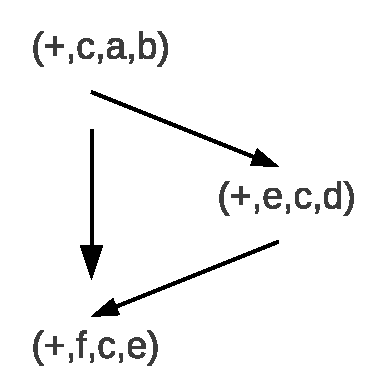
\includegraphics[width=60px]{gfx/dag_theory1}
 \caption{A simple, but fully connected, DAG.}
 \label{fig:dag_theory1}
\end{figure}


From such a DAG one can then now define a set of tasks that are ready, $R$, for exectuion as the nodes in the dag without any input edges.
\begin{equation*}
R = \forall n_i \in N \mid \{e_{*,t_i}\} = \emptyset,
\end{equation*}
where * matches any task.

Once a node is executed it is removed from the DAG, which in turn removes any edges from the node, which may enable other nodes to join the ready-set. If tasks are extended to include an execution time any given DAG may statically be reduced to a schedule which ensures maximum concurrency. Given however that the execution environment is distributed, the DAG must be extended to include localtion information. The location information could be mapped to the data elements, however if we assume that all data in a task must be located at the same execution element for it to perform we can also model the location on the tasks, which is what we choose to do here. Thus we define a list $L$ of locations of tasks:
\begin{equation*}
L={l_0,l_1,...,l_n}
\end{equation*}

Including the locations in the DAG we get a definition
\begin{equation*}
G=(N,E,M,L)
\end{equation*}


The DAG can then be, automatically, extended to include transfers from one task to another if the location of the two tasks are not placed at the same computing element.

\begin{equation*}
\forall e_{t_i,t_j} \in E \mid l_i \neq l_j : t_i,e_{t_i,t_j},t_j \mapsto t_i,e_{t_i,t_{new}},t_{new},e_{t_{new},t_j},t_j
\end{equation*}
where
\begin{equation*}
n_{new} = Transfer(dependency(D_j))
\end{equation*}
and
\begin{equation*}
dependency(D_j) = D_i \cap D_j \setminus dependency(D_i)
\end{equation*}
Thus if the previous example is extended to execute at three different locations, $[(\alpha,+,c,a,b),(\beta,+,e,c,d),(\delta, f,c,e)]$ translates into the DAG in figure \ref{fig:dag_theory2} and with the transfer nodes inserted in figure \ref{fig:dag_theory3}.


\begin{figure}
  \begin{center}
    \subfloat[\label{fig:dag_theory2}]{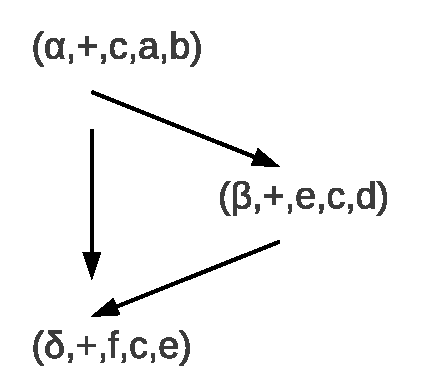
\includegraphics[width=60px]{gfx/dag_theory2}}
    \subfloat[\label{fig:dag_theory3}]{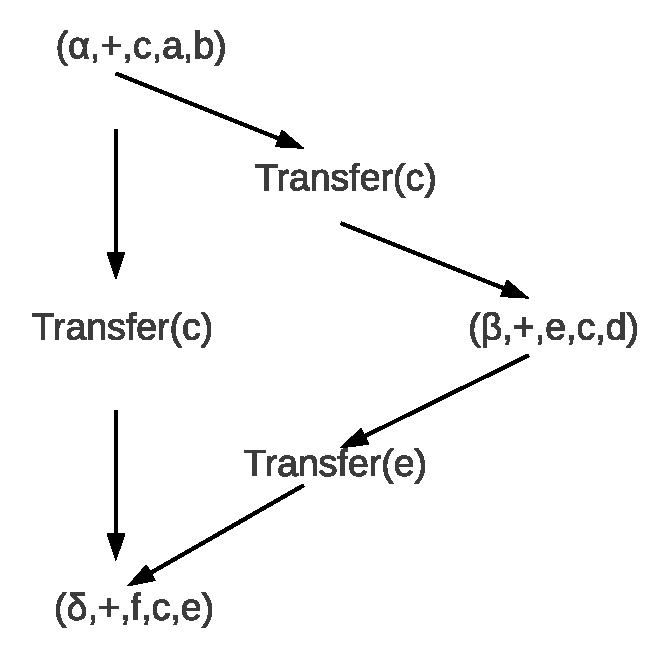
\includegraphics[width=115px]{gfx/dag_theory3}}
    \caption{A simple DAG, extended with locations.}
    \label{fig:MonteCarlo}
  \end{center}
\end{figure}





\section{Dependency Algorithm}


\section{Dependency Data Structure}



\section{Distributed Numerical Python as an Example}
The programming language Python combined with the numerical library NumPy\cite{numpy} has become a popular numerical framework amongst researchers. It offers a high level programming language to implement new algorithms that support a broad range of high-level operations directly on vectors and matrices.

The idea in NumPy is to provide a numerical extension to the Python language that enables the Python language to be both high productive and high performing. NumPy provides not only an API to standardized numerical solvers, but also a possibility to develop new numerical solvers that are both implemented and efficiently executed in Python, much like the idea behind the MATLAB\cite{guide1998mathworks} framework. 

DistNumPy is a new version of NumPy that parallelizes array operations in a manner completely transparent to the user -- from the perspective of the user, the difference between NumPy and DistNumPy is minimal. DistNumPy can use multiple processors through the communication library Message Passing Interface (MPI)\cite{mpi}. However, DistNumPy does not use the traditional single-program multiple-data (SPMD) parallel programming model because it requires the user to differentiate between the MPI-processes. Instead, the MPI communication in DistNumPy is fully transparent and the user needs no knowledge of MPI or any parallel programming model. 
The only difference in the API of NumPy and DistNumPy is the array creation routines. DistNumPy allow both distributed and non-distributed arrays to co-exist thus the user must specify, as an optional parameter, if the array should be distributed. The following illustrates the only difference between the creation of a standard array and a distributed array:
\lstset{frame=none, xleftmargin=0mm, numbers=none}
\begin{lstlisting}
#Non-Distributed
A = numpy.array([1,2,3])
#Distributed
B = numpy.array([1,2,3], dist=True)
\end{lstlisting}
\lstset{frame=single, xleftmargin=5mm, numbers=left}

\subsection{Views}
In DistNumPy an array does not necessarily represent a complete contiguous block of memory. An array is allowed to represent a subpart of another array i.e. it is possible to have a hierarchy of arrays where only one array represent a complete contiguous block of memory and the other arrays represent a subpart of that memory. DistNumPy implements an array hierarchy where distributed arrays are represented by the following two data structures.
\begin{itemize}
\item \textbf{Array-base} is the base of an array and has direct access to the content of the array in main memory. An array-base is created with all related meta-data when the user allocates a new distributed array, but the user will never access the array directly through the array-base. The array-base always describes the whole array and its meta-data such as array size and data type are constant.
\item \textbf{Array-view} is a view of an array-base. The view can represent the whole array-base or only a sub-part of the array-base. An array-view can even represent a non-contiguous sub-part of the array-base. An array-view contains its own meta-data that describe which part of the array-base is visible. The array-view is manipulated directly by the user and from the users perspective the array-view is simply a normal contiguous array.
\end{itemize}
Array-views are not allowed to refer to each other, which means that the hierarchy is flat with only two levels: array-base below array-view. However, multiple array-views are allowed to refer to the same array-base. This hierarchy is illustrated in Figure \ref{fig:views}. 

\begin{figure}
 \centering
 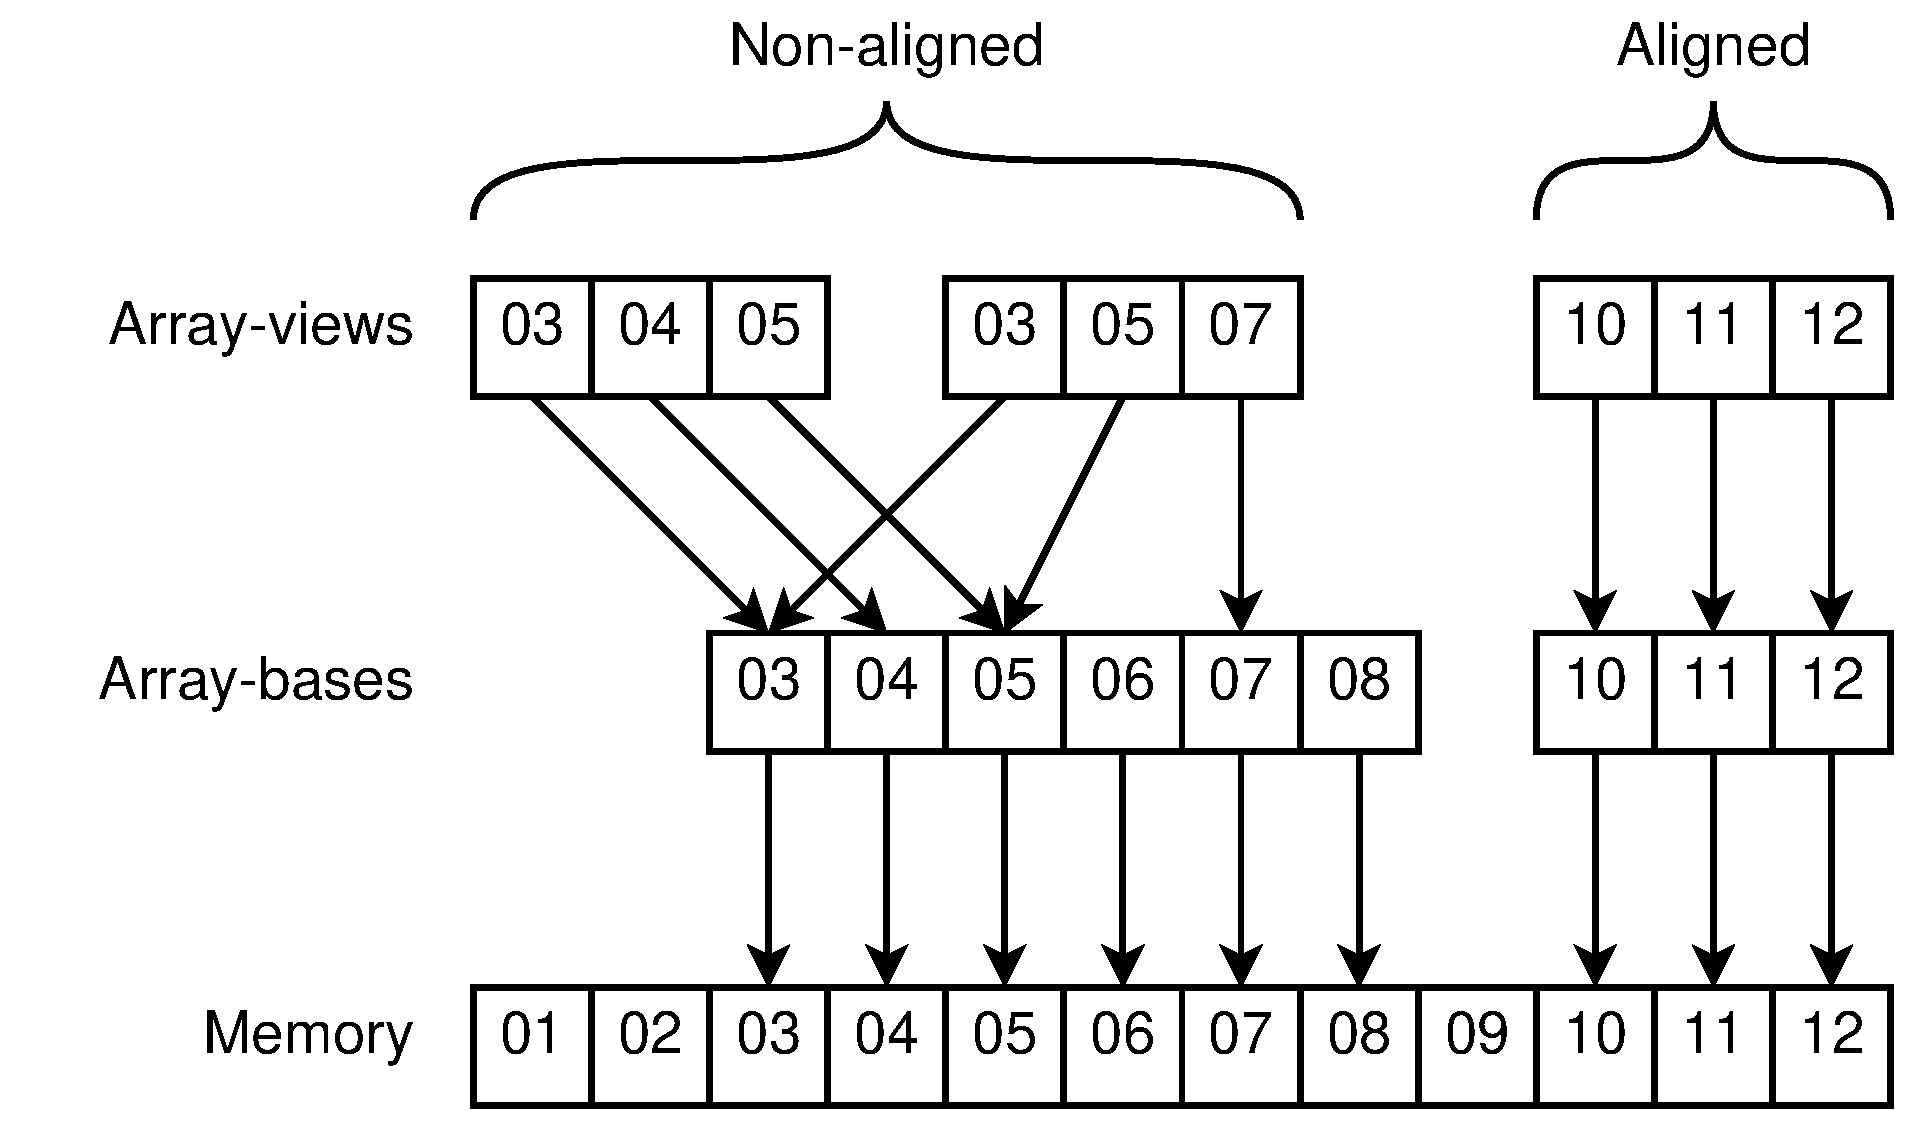
\includegraphics[width=\linewidth]{gfx/views}
 \caption{Reference hierarchy between the two array data structures and the main memory. Only the three array-views at top of the hierarchy are visible from the perspective of the user.}
 \label{fig:views}
\end{figure}

\section{Data Layout}
The data layout in DistNumPy consists of three kinds of data blocks: base-blocks, view-blocks and sub-view-blocks, which make up a three level abstraction hierarchy (Fig. \ref{fig:view_block}).

\begin{itemize}
\item \textbf{Base-block} is a block of an array-base and maps directly into one block of memory located on one node. The memory block is not necessarily contiguous but only one MPI-process has exclusive access to the block. Furthermore, DistNumPy makes use of a N-Dimensional Block Cyclic Distribution inspired by High Performance Fortran\cite{Loveman93}, in which base-blocks are distributed across multiple MPI-processes in a round-robin fashion.


\item \textbf{View-block} is a block of an array-view and from the perspective of the user a view-block is a contiguous block of array elements. A view-block can span over multiple base-blocks and consequently also over multiple MPI-processes. For a MPI-process to access a whole view-block it will have to fetch data from possible remote MPI-processes and put the pieces together before accessing the block. To avoid this process, which may cause some internal memory copying, we divide view-blocks into sub-view-block.

\item \textbf{Sub-view-block} is a block of data that is a part of a view-block but is located on only one MPI-process. The driving idea is that all array operation is translated into a number of sub-view-block operations.

\end{itemize}

%The data layout that DistNumPy uses consists of three levels . The first level is the base-block level, in which a base-block map directly into one block of memory located on one node. The memory block is not necessarily contiguous but only one MPI-process has exclusive access to the block. DistNumPy makes use of a N-Dimensional Block Cyclic Distribution inspired by High Performance Fortran\cite{Loveman93}, in which base-blocks are distributed across multiple MPI-processes in a round-robin fashion.

%The second level is the view-block level, which is an abstraction level above the base-block level. A view-block represents a basic block of an array-view, which means that a view-block is a contiguous block of array elements from the perspective of the user. A view-block can span over multiple base-blocks and consequently also over multiple MPI-processes. For a MPI-process to access a whole view-block it will have to fetch data from possible remote MPI-processes and put the pieces together before accessing the block. To avoid this process, which may require some internal memory copying, we divide view-blocks into sub-view-block.

%Sub-view-block is the third block level and is simply a block of data that is a part of a view-block but is located on only one MPI-process. The general idea is that all array operation is translated into a number of sub-view-block operations.

We will define an \emph{aligned array} as an array that have a direct contiguous mapping through the block hierarchy. That is, a distributed array in which the base-blocks, view-blocks and sub-view-blocks are identical. A \emph{non-aligned array} is then a distributed array without this property.

\begin{figure}
 \centering
 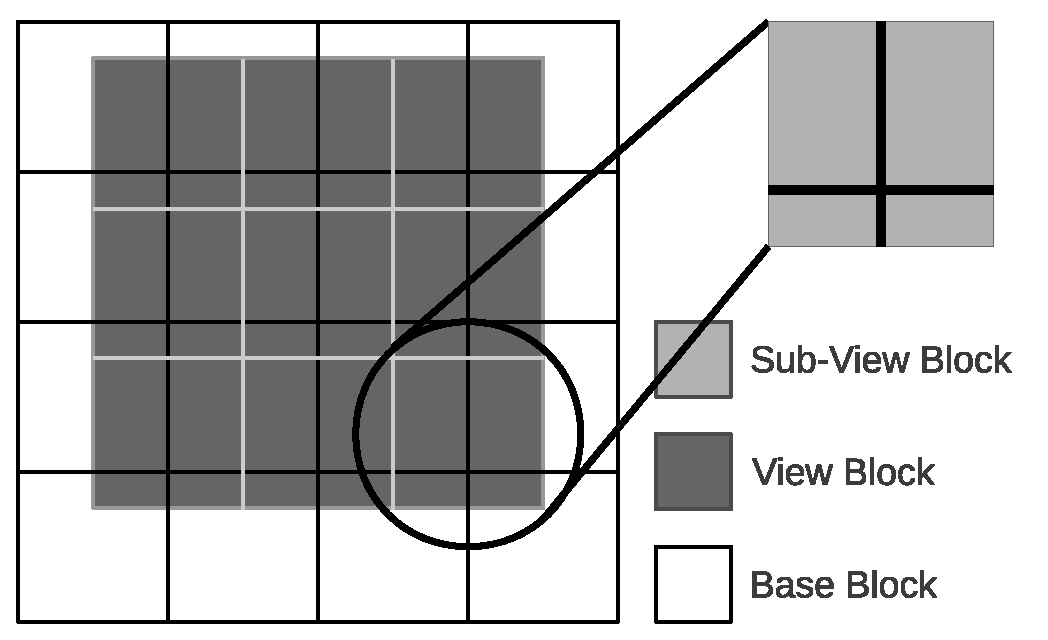
\includegraphics[width=150px]{gfx/view_blocks}
 \caption{An illustration of the block hierarchy that represents a 2D distributed array. The array is divided into three block-types: Base, View and Sub-View-blocks. The 16 base-blocks make up the base-array, which may be distributed between multiple MPI-processes. The 9 view-blocks make up a view of the base-array and represent the elements that are visible to the user. Each view-block is furthermore divided into four sub-view-blocks, each located on a single MPI-process.}
 \label{fig:view_block}
\end{figure}


\section{Universal Function}
An important mechanism in DistNumPy is a concept called Universal function. A universal function (ufunc) is a function that operates on all elements in an array-view independently. That is, an ufunc is a vectorized wrapper for a function that takes a fixed number of scalar inputs and produces a fixed number of scalar outputs. E.g., addition is an ufunc that takes three array-views as argument: two input arrays and one output array. For each element, the ufunc adds the two input arrays together and writes the result into the output array. Using ufunc can result in a significant performance boost compared to native Python because the computation-loop is implemented in C and is executed in parallel.

Applying an ufunc operation on a whole array-view is semantically equivalent to performing the ufunc operation on each array-view block individually. This property makes it possible to perform a distributed ufunc operation in parallel. 

A distributed ufunc operation consists of four steps:
\begin{enumerate}
\item All MPI-processes determents the distribution of the view-block computation, which is strictly based on the distribution of the output array-view.
\item All MPI-processes exchange array elements in such a manner that all MPI-processes can perform its computation locally. 
\item All MPI-processes performs its local computation.
\item All MPI-processes sends the written array elements back to the original locations.
\end{enumerate}



\section{Latency Hiding}
\begin{figure}
 \centering
 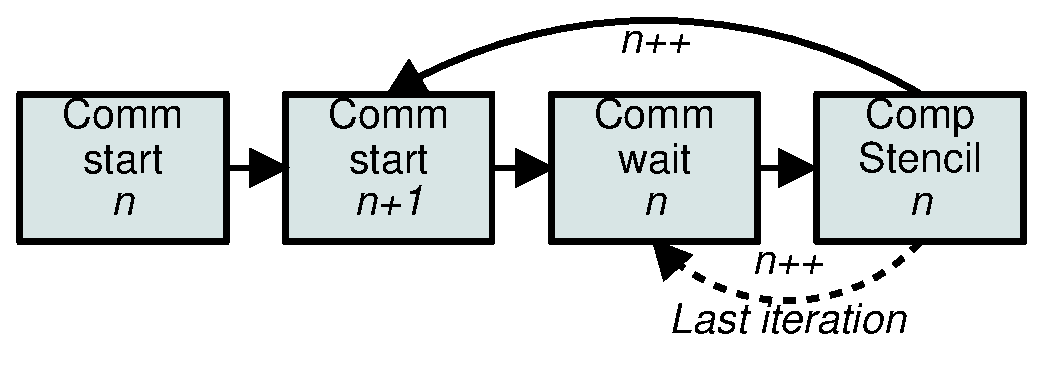
\includegraphics[width=200px]{gfx/double_buffering}
 \caption{Flow diagram illustrating double buffering. The $n$'th iteration is expressed with a $n$ and Comm and Comp represents communication and computation, respectively. $n$++ is an iteration to $n$'s successor.}
 \label{fig:double_buffering}
\end{figure}

The standard approach to hide communication latency behind computation in message-passing is a technique known as double buffering. The implementation of double buffering is straightforward when operating on a set of data block that all have identical sizes. The communication of one data block is overlapped with the computation of another already communicated data block (Fig. \ref{fig:double_buffering}) and since the sizes of all the data blocks are identical all iterations are identical.

The current version of DistNumPy makes use of the straightforward double buffering approach. It works very well for ufuncs that operates on aligned arrays because it translates into communication and computation operations on whole view-blocks, which does not benefited from latency hiding inside a view-blocks. However, for ufuncs that operates on non-aligned arrays this is not the case because the view-block is distributed between multiple MPI-processes. 

In order to achieve good performance when operating on non-aligned arrays the implementation must introduces some latency hiding inside view-blocks. For example the computation of a view-block in figure \ref{fig:view_block} can make use of latency hiding by first initiate the communication of the three non-local sub-view-blocks, then compute the local sub-view-block and finally compute the three communicated sub-view-blocks. 

What we need is a generic approach that, based on the executing program, schedules the communication and computation in an overlapping pattern. Since Python is an interpreted dynamic programming language, it is not possible to schedule communication and computation operation at compile time. Instead some kind of a lazy evaluation technique is required to determine the communication and computation operations used in the program at runtime.


\section{Lazy Evaluation}
To make it possible for a scheduler to schedule communication behind computation operations we introduce Lazy Evaluation. During the execution of a DistNumPy program all MPI-processes records the requested array operations rather than applying them immediately. We maintain the operations in a convenient data structure and at a later point all MPI-processes applies the operations. The idea is that by having a bunch of operations to carry out it may be possible to schedule communication and computation operations that have no mutual dependencies in parallel.

We will only introduce lazy evaluation for Python operations that involve DistNumPy arrays. The Python interpreter executes Python operations that do not include DistNumPy arrays immediately. Thus, the interpreter will also have to execute DistNumPy operations that involve program branches immediately because a branch may lead to non-DistNumPy operations. This means that when we encounter a branch the interpreter will execute all previously recorded operations. This mechanism of executing all previously recorded operation we will call an \emph{operation flush}. The two only other conditions that can trigger an operation flush is when the number of recorded operations reaches a user-defined threshold or when the Python interpreter reaches the end of the program. Furthermore, an operation flush always include all recorded operations.


\subsection{The Dependency System}
The main challenge when introducing Lazy Evaluation is to implement a dependency system that schedules operations in a performance efficient manner while the implementation keeps the overhead at an acceptable level.

The partial order of operations imposed by operational dependencies is normally represented by a directed acyclic graph (DAG)\cite{AhSeUl86}. The nodes of the DAG represent operations and the edges represent the dependencies between the operations. E.g. a DAG with two nodes $A$ and $B$ and an edge from $A$ to $B$ means that $A$ must be executed before $B$ to preserve correctness of the overall program. 

Our first lazy evaluation approach makes use of a DAG to contain all recorded operations. When an operation is recorded, it is split across the sub-view-blocks that are involved in the operation. For each such operation, a DAG node is created. Figure \ref{lst:code_eg}  is an illustration of a small Python program and figure \ref{fig:DAG} is the corresponding DAG.
 
Beside the DAG our dependency system also consist of a \emph{ready queue}, which is a queue of recorded operations that do not have any dependencies. The ready queue makes it possible in to find operations that are ready to be executed in the time complexity of $O(1)$.

\begin{figure}
\begin{lstlisting}
import numpy
base = numpy.array([1,2,3,4,5],dist=True)
A = base[:2]    #A = [1,2]
R = base[2]     #R = [3]
B = base[3:]    #B = [4,5]
T = A + B       #T = [5,7]
R = T[1] * B[0] #R = [28]
print base      #out: [1,2,28,4,5]
\end{lstlisting}
 \caption{This is an example of a small Python program that makes use of DistNumPy.}
 \label{lst:code_eg}
\end{figure}

\begin{figure}
 \centering
 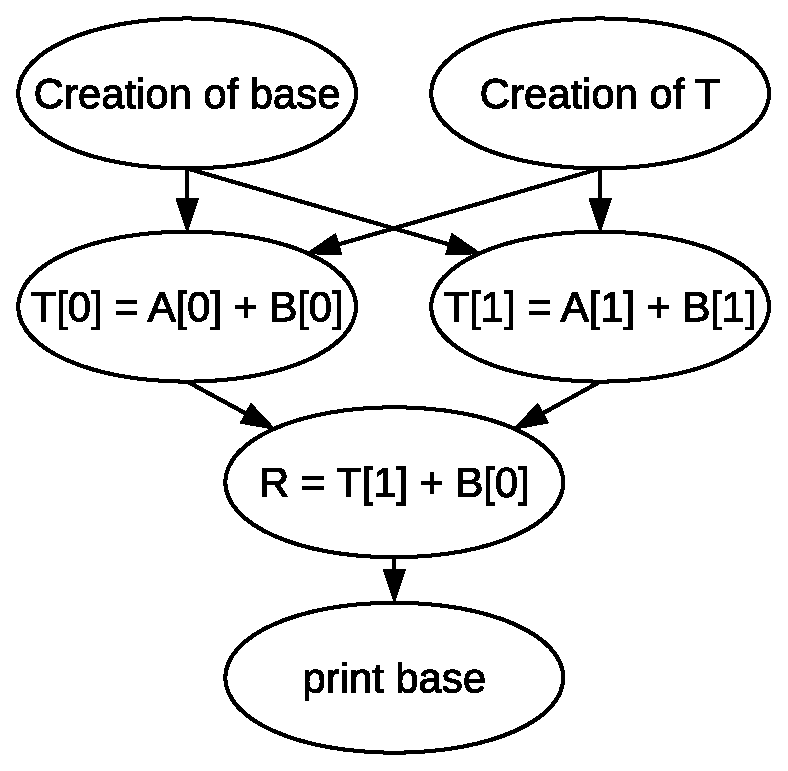
\includegraphics[width=120px]{gfx/dag}
 \caption{This figure illustrates a directed acyclic graph that represents the operational dependencies in figure \ref{lst:code_eg}. The block size is in this case is one and the numbers inside brackets are references to specific blocks. Note that a block size of one entails that base-blocks, view-blocks and sub-view-blocks all are identical. Note that there are no creation nodes for \texttt{A}, \texttt{R} and \texttt{B} since they are only views of \texttt{base}.}
 \label{fig:DAG}
\end{figure}


\subsubsection{Operation Insertion}
The recording of an operation triggers an insertion of new node into the DAG. A straightforward approach will simply implement insertion by comparing the new node with all the nodes already located in the DAG. If a conflict is detected the implementation added an edge between the two conflicting nodes. The time complexity of such an implementation is $O(n)$ where $n$ is the number of operation in the DAG and the construction of the complete DAG is $O(n^2)$.

%In worse case this approach is optimal because the longest path through the DAG is always $n$. However, we have introduced some heuristics to speed up the common case. 

\subsubsection{Operation Flush}
To archive good performance the operation flush implementation must maximize the amount of communication that it is hiding behind computation. Our approach to achieve this is to initiate communication at the earliest point in time and only do computation when all communication has been initiated. Furthermore, to make sure that there is progress in the MPI layer we check for finished communication in between multiple computation operations. The following is the flow of our operation flush algorithm:
\begin{enumerate}
\item Initiate all communication operation in the ready queue.
\item Check in a non-blocking manner if some communication operations have finished and remove possible finished communication operations from the ready queue and the DAG. Furthermore, register operations that now have no dependencies into the ready queue.
\item If there is only computation operations in the ready queue execute one of them and remove it from the ready queue and the DAG.
\item Go back to step one if there is any operation left in the ready queue else we are finished.
\end{enumerate}
The algorithm maintains the following three invariants:
\begin{enumerate}
\item All operations, that are ready, are located in the ready queue.
\item We only start the execution of a computation node when there is no communication node in the ready queue.
\item We only wait for communication when the ready queue has no computation nodes.
\end{enumerate}



\subsubsection{Dependency Heuristic}
Experiments with lazy evaluation using the dependency DAG shows that the overhead associated with the creation of the DAG is very time consuming and becomes the dominating performance factor. In the worse case this is the best solution, however we introduce a heuristic to speed up the common case. 

We base the heuristic on the observation that in the common case a program spreads a computation evenly between all sub-view-blocks in the involved arrays and that it is only possible to have conflicts between sub-view-blocks that are part of the same base-block. The heuristic is that instead of having one DAG only, we introduce a DAG for each base-block -- the assumption is that in the common case heuristic will dramatically reduce the size of each DAG. Actually, we expect the size of the DAGs to be at a level where it makes most sense to use a linked list rather than a more complex DAG.


\subsubsection{The non-DAG approach}
The approach we end up using does not use any DAGs -- instead a number of operation-nodes and access-nodes represent the operation dependencies. An operation-node contains all information need to execute the operation on a set of sub-view-blocks and there is a pointer to an access-node for each sub-view-block. Access-nodes represent memory access to a sub-view-block, which can be either reading or writing. E.g., the representation of an addition operation on three sub-view-blocks is two read access-nodes and one write access-node. 

Our approach places all access-nodes in dependency-lists based on the base-block that they are accessing. Figure \ref{fig:dependency_system_term} goes through all the structures that make up our dependency system.

%An operation is said to be ready for execution when none of its sub-view-block access conflicts with any earlier recorded access.  

\def\imagetop#1{\vtop{\null\hbox{#1}}}
\begin{figure}
 \centering
\begin{tabular}{cp{165px}}
\imagetop{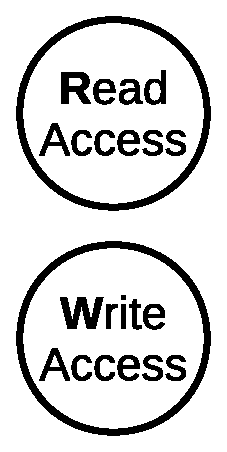
\includegraphics[width=30px]{gfx/dependency_system_access}} & \vspace{1px} All access-nodes that access the same base-block are linked together in a dependency-list. The order of the list is simply based on the time of node insertion (descending order). Additionally an access-node contains the information needed to determine whether it conflict with other access-nodes.\newline \\
\imagetop{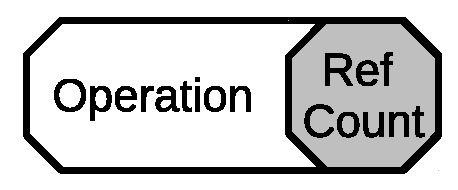
\includegraphics[width=50px]{gfx/dependency_system_op}} & An operation-node has a pointer to all access-nodes that are involved in the operation and attached to an operation is a reference counter that specifies the number of conflicts associated with the operation. When the counter reach zero the operation is ready for execution. At some point when the operation has been executed the operation-node and all access-nodes are completely remove from the dependency system.\\
\imagetop{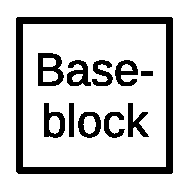
\includegraphics[width=28px]{gfx/dependency_system_block}} & \vspace{3px} A base-block simply contains a pointer to the first access-node in the dependency-list.\\
\end{tabular}
 \caption{dependency system term}
 \label{fig:dependency_system_term}
\end{figure}



\begin{figure}
 \centering
 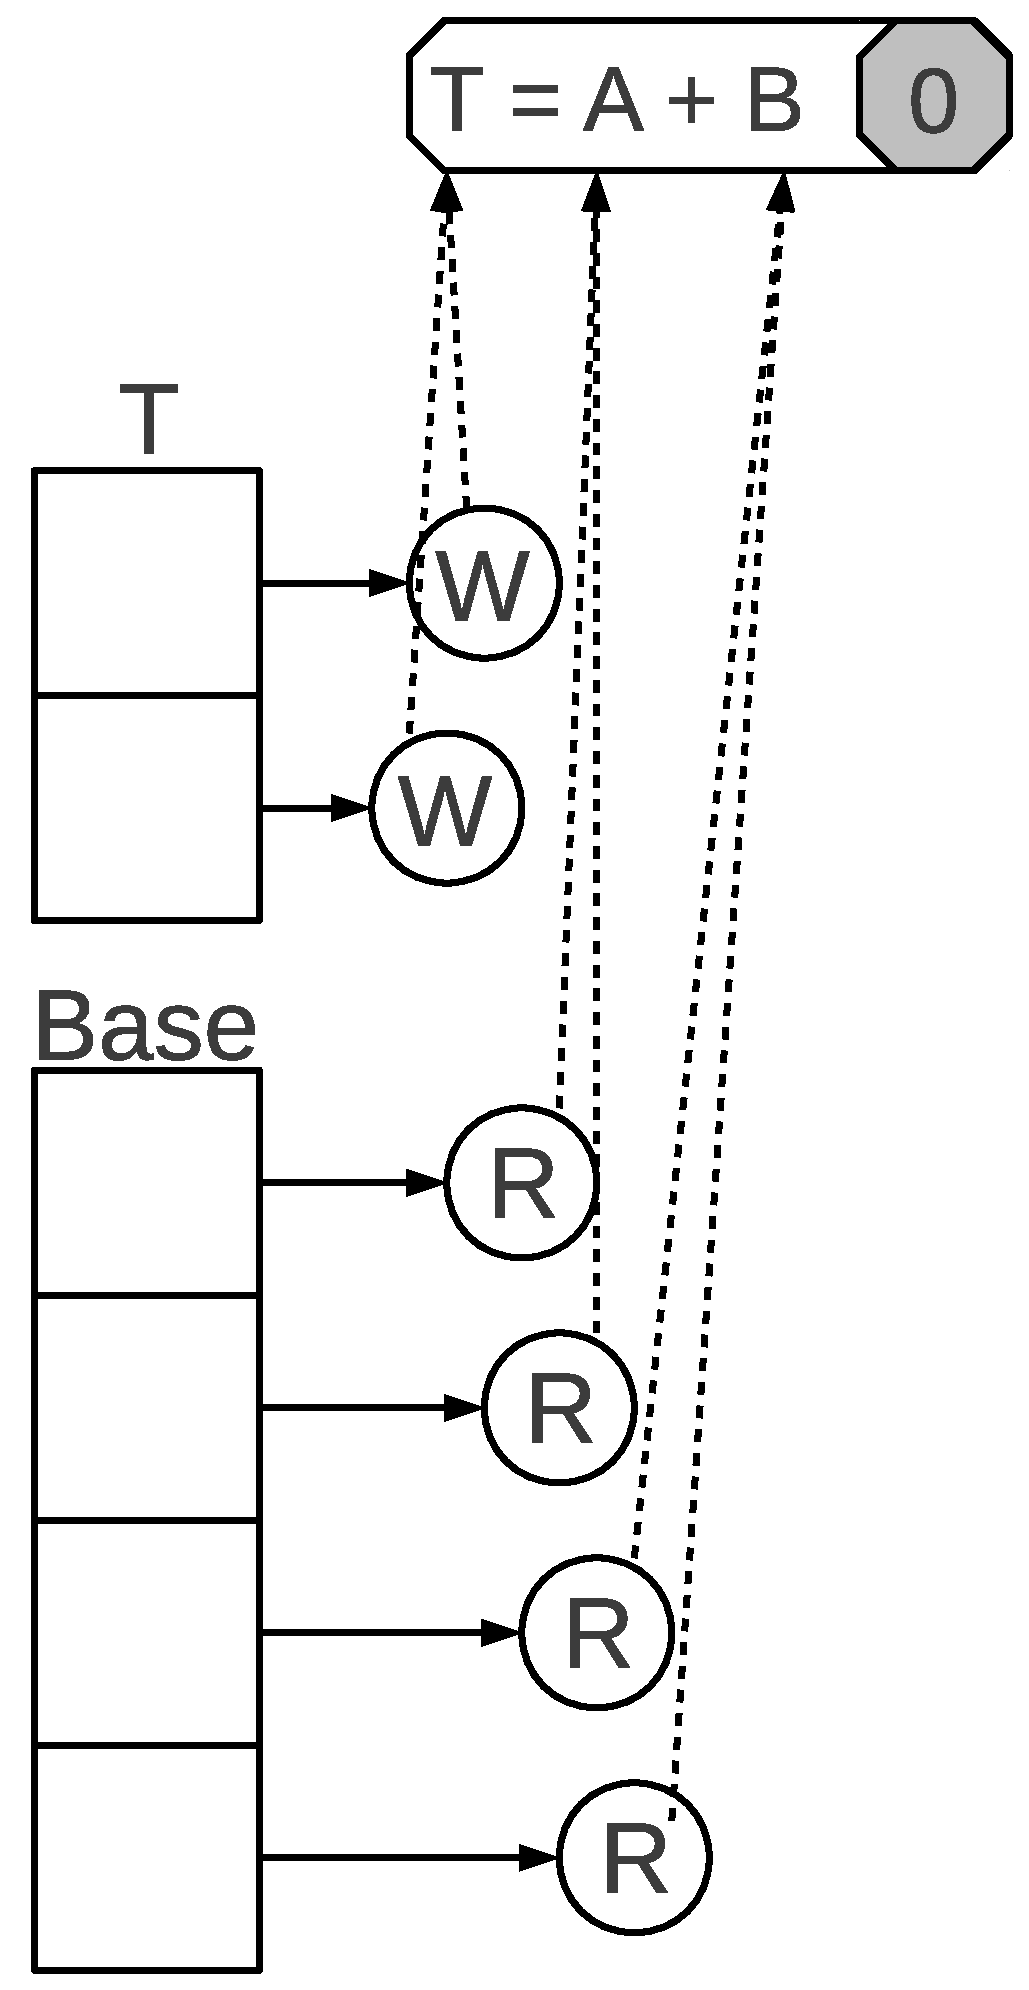
\includegraphics[width=\linewidth]{gfx/dependency_system}
 \caption{dependency system}
 \label{fig:dependency_system}
\end{figure}

%Lazy evaluation on these data blocks are managed through a simple dependency list for each block. When a NumPy operation is issued it is split across the sub-view blocks that are involved in the operation. For each such operation on a sub-view block a set of tasks are created, one for each combined set of data-blocks to sub-view blocks. Dependencies are then added to the dependency-list of each data-block that is involved, each dependency link back to the individual tasks. When the number of dependencies on a task reached zero the task may be moved to the ready-queue. But before this is done we traverse the dependency list and include any other task that can be merged into the ready task, given that they could execute in parallel with the task or could execute given the task was done, when two tasks are merged into one, the remaining list is traversed under the same rules but for the merged task.


\subsection{Ufunc Operation List}




\section{Examples}


\section{Experiments}


\section{Future work}


\section{Conclusions}


\bibliographystyle{abbrv}
\bibliography{/home/madsbk/repos/priv/diku/phd/paper_archive/main}




\end{document}